%==============================================================================
% Chapitre 66 - Que se passe-t-il lorsque l'on appuie sur la détente ?
%==============================================================================

\section{Introduction}

Les chapitres précédents ont présenté les principaux composants des armes et
des munitions.

Nous allons maintenant étudier les phénomènes qui se produisent lors du tir.

Ces phénomènes se déroulent extrêmement rapidement, généralement en quelques
millisecondes seulement.

Pourtant, ils déterminent une grande partie des performances de l'ensemble
arme-munition.

\begin{aretenir}

La balistique intérieure étudie les phénomènes qui se produisent entre la
percussion de l'amorce et la sortie du projectile de la bouche du canon.

\end{aretenir}

\section{Une succession d'événements}

Le départ d'un coup n'est pas un événement unique.

Il s'agit d'une succession très rapide de phénomènes physiques étroitement
liés les uns aux autres.

\begin{figure}[htbp]
\centering

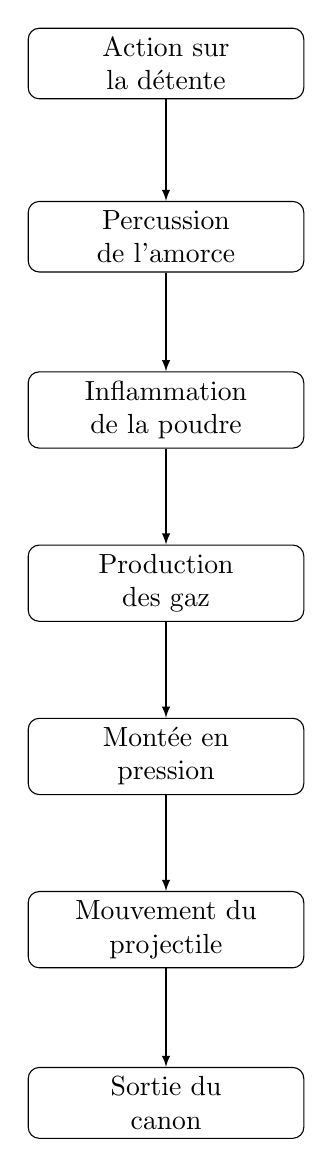
\begin{tikzpicture}[
every node/.style={
draw,
rounded corners,
align=center,
minimum width=3.5cm
}
]

\node (D) at (0,0)
{Action sur\\la détente};

\node (P) at (0,-2.2)
{Percussion\\de l'amorce};

\node (A) at (0,-4.4)
{Inflammation\\de la poudre};

\node (G) at (0,-6.6)
{Production\\des gaz};

\node (Pr) at (0,-8.8)
{Montée en\\pression};

\node (M) at (0,-11)
{Mouvement du\\projectile};

\node (S) at (0,-13.2)
{Sortie du\\canon};

\draw[-latex] (D) -- (P);
\draw[-latex] (P) -- (A);
\draw[-latex] (A) -- (G);
\draw[-latex] (G) -- (Pr);
\draw[-latex] (Pr) -- (M);
\draw[-latex] (M) -- (S);

\end{tikzpicture}

\caption{Principales étapes du départ du coup.}
\label{fig:chronologie_depart_coup}

\end{figure}

\section{Action sur la détente}

Le processus débute lorsque le tireur agit sur la détente.

Cette action provoque la libération du mécanisme de percussion.

\section{Percussion de l'amorce}

Le percuteur frappe l'amorce avec une énergie suffisante pour provoquer son
fonctionnement.

L'amorce produit alors une flamme et des gaz chauds.

\section{Inflammation de la poudre}

La flamme issue de l'amorce pénètre dans l'étui et atteint la charge de poudre.

La combustion débute alors.

\section{Production des gaz}

La combustion transforme progressivement une partie de la poudre en gaz.

Ces gaz occupent un volume beaucoup plus important que les matériaux dont ils
proviennent.

\section{Montée en pression}

Comme le projectile est encore immobilisé dans la cartouche ou dans le canon,
les gaz ne peuvent pas se détendre librement.

La pression augmente donc rapidement.

\section{Début du mouvement du projectile}

Lorsque la pression devient suffisante, le projectile commence à se déplacer.

Cette mise en mouvement marque une étape importante du cycle de tir.

\section{Accélération dans le canon}

Le projectile est accéléré tout au long de son déplacement dans le canon.

La pression des gaz continue à agir sur sa base.

\section{Évolution simultanée des phénomènes}

Pendant le déplacement du projectile :

\begin{itemize}
    \item la poudre continue à brûler ;
    \item la quantité de gaz augmente ;
    \item le volume disponible évolue ;
    \item la pression varie.
\end{itemize}

Tous ces phénomènes se produisent simultanément.

\section{Sortie du projectile}

Lorsque le projectile atteint l'extrémité du canon, il quitte l'arme.

La phase de balistique intérieure prend alors fin.

\section{Début de la balistique extérieure}

Après la sortie du canon, le projectile poursuit son déplacement dans l'air.

L'étude de cette nouvelle phase relève de la balistique extérieure.

\begin{figure}[htbp]
\centering

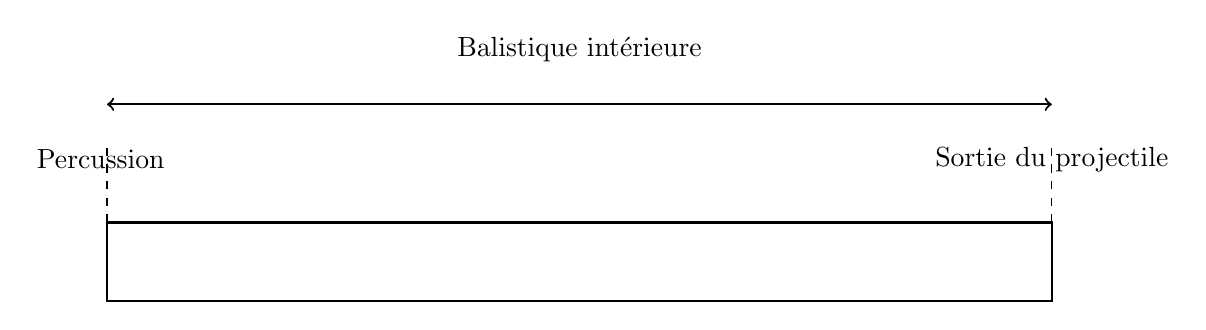
\begin{tikzpicture}

% Canon
\draw[thick]
(0,0)
rectangle
(12,1);

\node at (-0.08,1.8)
{Percussion};

\node at (12,1.8)
{Sortie du projectile};

\draw[dashed]
(0,1)
--
(0,2);

\draw[dashed]
(12,1)
--
(12,2);

\draw[<->,thick]
(0,2.5)
--
(12,2.5);

\node at (6,3.2)
{Balistique intérieure};

\end{tikzpicture}

\caption{La balistique intérieure s'étend de la percussion à la sortie du projectile.}
\label{fig:limites_balistique_interieure}

\end{figure}

\begin{figure}[htbp]
\centering

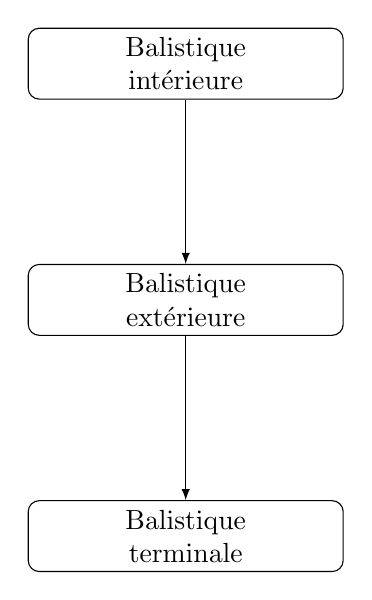
\begin{tikzpicture}[
every node/.style={
draw,
rounded corners,
align=center,
minimum width=4cm
}
]

\node (I) at (0,0)
{Balistique\\intérieure};

\node (E) at (0,-3)
{Balistique\\extérieure};

\node (T) at (0,-6)
{Balistique\\terminale};

\draw[-latex] (I) -- (E);
\draw[-latex] (E) -- (T);

\end{tikzpicture}

\caption{Les trois principaux domaines de la balistique.}
\label{fig:trois_domaines_balistique}

\end{figure}

\section{Durées caractéristiques}

L'ensemble des phénomènes décrits précédemment se déroule généralement sur des
durées extrêmement courtes.

Selon l'arme et la munition, le cycle complet représente souvent quelques
millisecondes seulement.

\begin{figure}[htbp]
\centering

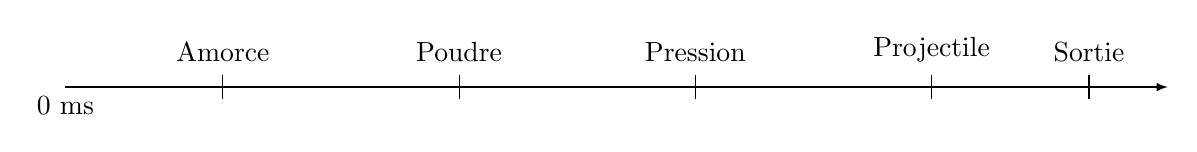
\begin{tikzpicture}

% Axe du temps
\draw[-latex]
(0,0)
--
(14,0);

\node[below]
at (0,0)
{0 ms};

\draw (2,0.15) -- (2,-0.15);
\node[above]
at (2,0.2)
{Amorce};

\draw (5,0.15) -- (5,-0.15);
\node[above]
at (5,0.2)
{Poudre};

\draw (8,0.15) -- (8,-0.15);
\node[above]
at (8,0.2)
{Pression};

\draw (11,0.15) -- (11,-0.15);
\node[above]
at (11,0.2)
{Projectile};

\draw (13,0.15) -- (13,-0.15);
\node[above]
at (13,0.2)
{Sortie};

\end{tikzpicture}

\caption{Les phénomènes de balistique intérieure se déroulent en quelques millisecondes.}
\label{fig:temps_balistique_interieure}

\end{figure}

\section{Pourquoi cette phase est importante}

La balistique intérieure détermine notamment :

\begin{itemize}
    \item la vitesse initiale ;
    \item les contraintes mécaniques ;
    \item le recul ;
    \item les performances générales du tir.
\end{itemize}

\section{Une discipline fortement instrumentée}

La compréhension de ces phénomènes nécessite souvent l'emploi
d'instrumentations spécialisées :

\begin{itemize}
    \item capteurs de pression ;
    \item chronographes ;
    \item caméras rapides ;
    \item systèmes d'acquisition.
\end{itemize}

\begin{simulation}

Dans un simulateur, les phénomènes de balistique intérieure sont généralement
représentés par des modèles mathématiques simplifiés.

Le calcul détaillé de chaque réaction chimique serait souvent trop coûteux en
temps de calcul.

Les simulateurs utilisent donc des modèles permettant d'estimer l'évolution de
la pression, de la vitesse et de l'accélération du projectile.

\end{simulation}

\begin{figure}[htbp]
\centering

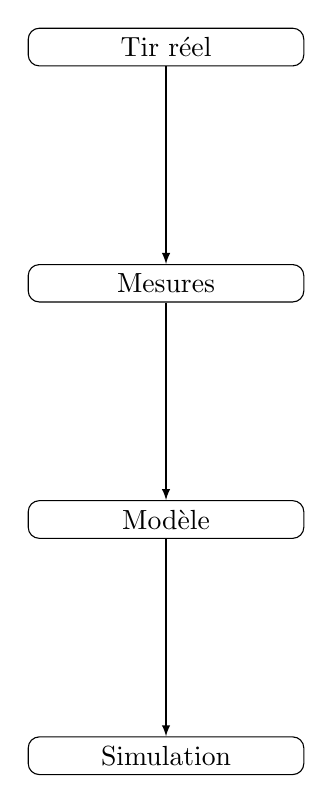
\begin{tikzpicture}[
every node/.style={
draw,
rounded corners,
align=center,
minimum width=3.5cm
}
]

\node (R) at (0,0)
{Tir réel};

\node (M) at (0,-3)
{Mesures};

\node (Mo) at (0,-6)
{Modèle};

\node (S) at (0,-9)
{Simulation};

\draw[-latex] (R) -- (M);
\draw[-latex] (M) -- (Mo);
\draw[-latex] (Mo) -- (S);

\end{tikzpicture}

\caption{Principe général de construction d'un modèle de simulation.}
\label{fig:essais_modele_simulation}

\end{figure}

\section{Vers l'étude détaillée des phénomènes}

Nous avons décrit ici la succession générale des événements.

Les chapitres suivants examineront chacun de ces phénomènes de manière plus
approfondie.

\section{À retenir}

\begin{aretenir}

\begin{itemize}
    \item La balistique intérieure débute avec la percussion de l'amorce.
    \item La combustion de la poudre produit des gaz sous pression.
    \item Cette pression accélère le projectile dans le canon.
    \item Tous les phénomènes évoluent simultanément.
    \item La balistique intérieure se termine à la sortie du projectile.
\end{itemize}

\end{aretenir}
